\section{A Linked List using Fine-Grained Locking}

We now consider another application of fine-grained locking, namely a linked
list, where each node in the list can be locked independently.  In particular,
we will use a linked list to implement a set containing values of some
type~|A|, following the trait in Figure~\ref{fig:Set-trait}.

Each node in the linked list will contain an immutable |datum| field of
type~|A|, representing a value in the set, and a |next| reference to the next
node in the list, or |null| in the case of the last node in the list.  To make
things easier, we will use a dummy header node, whose |datum| is not part of
the represented set: this will ensure that every proper node has a
predecessor, and so allows a uniform approach, meaning we don't have to treat
the first node as a special case.

We will keep the list ordered by |datum| fields.  This means that, in most
applications, on average we will only have to search about half way through
the list for a particular value.  For this to work, we need an order relation
over |A|.  The class signature in Figure~\ref{fig:LinkedListSet} captures
this.  The trait |Ordered[A]| represents an order relation over~|A|, allowing
us to use operations such as |<|.  The class signature requires there to be a
function |ord| that, given a value in~|A|, returns a value in |Ordered[A]|
that can be compared.  This function is provided \emph{implicitly}: when
creating an instance of the class, the Scala compiler will instantiate
automatically |ord| if it can; it is able to do this for many types, such as
|Int| or |Double|.  Likewise, |ord| is applied implicitly when it is necessary
to compare two elements of type~|A|.

The |Node| class in Figure~\ref{fig:LinkedListSet} defines the nodes from
which the linked list is built.  Each node has its own |Lock|, which is used
to protect the |next| field.  For convenience, we provide |lock| and |unlock|
operations, to lock or unlock a node.  The variable |header| holds the dummy
header node. 
%
The |LinkedListSet| object represents the set of |datum| fields of nodes
reachable from |header| by following one or more |next| references.

%%%%%

\begin{figure}
\begin{scala}
class LinkedListSet[A](implicit ord: A => Ordered[A]) extends Set[A]{
  /** Nodes from which the linked list is constructed.  Any access to the £next£ 
    * field must be done while holding the lock on this node.  */
  private class Node(val datum: A, var next: Node){
    /** A lock used to protect the £next£ field. */
    private val l = new Lock

    /** Lock this node. */
    def lock() = l.acquire()

    /** Unlock this node. */
    def unlock() = l.release()
  }

  /** A dummy header node. */
  private val header = new Node(null.asInstanceOf[A], null)

  /* Datatype invariant: the nodes from £header.next£ onwards are in strictly
   * increasing order of £datum£ fields. */ 

  ... // Continued in Figure £\ref{fig:LinkedListSet2}£.
}
\end{scala}
\caption{Outline of the linked list implementation.}
\label{fig:LinkedListSet}
\end{figure}

%%%%%

Let's review how the operations on a linked list work in a sequential
implementation.  The |contains(x)| operation traverses the list until either
it finds a node~|n| with $\sm{n.datum} \ge \sm x$, or it reaches the end of
the list; it returns true if it reached a node with $\sm{n.datum} = \sm x$.

The |add(x)| operation traverses the list until it finds a node~|p| such that
$\sm{p.next} = \sm{null}$ or $\sm{p.next.datum} \ge \sm{x}$.  In the case that
$\sm{p.next.datum} \ne \sm{x}$, it inserts a new node containing~|x|
after~|p|.  This is depicted in Figure~\ref{fig:linkedlist-ops} (left).

%%%%%

\begin{figure}
\def\new{red} % colour to depict updates.
\tikzstyle{every node}=[minimum height = 5mm, minimum width = 5mm]
\begin{center}
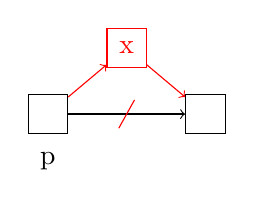
\begin{tikzpicture}[xscale = 2, yscale = 1.2]
\draw (0,0) node[draw] (p) { }; \draw (p)++(0,-0.5) node{\sm p};
\draw (p)++(1,0) node[draw] (n) { }; \draw[->] (p) -- (n);
% new node
\draw (p)++(0.5,0.7) node[draw,\new] (new) {\mbox{\scalastyle\color{\new} x}};
\draw[->, \new] (p) -- (new); \draw[->, \new] (new) -- (n);
\draw[\new] (p)++(0.45,-0.15) -- ++(0.1,0.3);
\end{tikzpicture}
%
\hfil
%
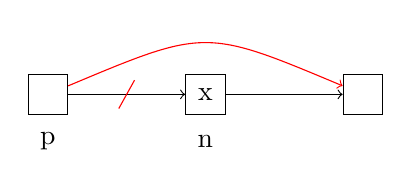
\begin{tikzpicture}[xscale = 2, yscale = 1.2]
\draw (0,0) node[draw] (p) { }; \draw (p)++(0,-0.5) node{\sm p};
\draw (p)++(1,0) node[draw] (n) {\sm x};  \draw (n)++(0,-0.5) node{\sm n};
\draw[->] (p) -- (n);
\draw (n)++(1,0) node[draw] (next) { }; \draw[->] (n) -- (next);
% updates
\draw[->, \new] (p) .. controls (1.0,0.7) .. (next);
\draw[\new] (p)++(0.45,-0.15) -- ++(0.1,0.3);
\end{tikzpicture}
\end{center}
\caption{Operations on a linked list: adding a node (left), and removing a node
  (right).}
\label{fig:linkedlist-ops}
\end{figure}

%%%%%

The |remove(x)| operation traverses the list until it finds a node~|p| such that
$\sm{p.next} = \sm{null}$ or $\sm{p.next.datum} \ge \sm{x}$.  In the case that
$\sm{p.next.datum} = \sm{x}$, it updates |p.next| to point to |n.next|.  This
is depicted in Figure~\ref{fig:linkedlist-ops} (right).

What about concurrency?  We will take the linearization points of a successful
|add| or |remove| operation to be the point at which the relevant |next| field
is updated.  First, note that when a thread~$t$ updates |p.next|, to insert or
delete a node, $t$ should have~|p| locked.  Otherwise there is an obvious race
condition: two threads could update |p.next| concurrently, and one of those
updates would be lost.  Also, $t$ should lock~|p| before reading its |next|
field, to avoid races.  Further, when deleting a node~|n|, thread~$t$ should
lock~|n| and read its |next| field first: otherwise, another thread could
update |n.next| after~$t$ has read it, and that latter update would be lost.

It is also necessary to perform locking while traversing the list, searching
for the relevant node.  If not it is possible for a thread~$t$ to find the
relevant predecessor node~|p|, but for another thread to delete~|p| before $t$
locks it.  This would mean that $t$'s updates would be lost.


%%%%%

\begin{figure}
\begin{scala}
  /** Find the first node £p£ that such that £p.next = null£ or £p.next.datum $\ge$ x£.
    * £p£ will be locked on return, and not removed from the list. */  
  private def find(x: A): Node = {
    var p = header; p.lock()
    // Invariant: all nodes £n£ before £p£ have £n.next.datum $<$ x£; £p£ is locked 
    // and in the linked list.
    while(p.next != null && p.next.datum < x){
      val n = p.next; n.lock(); p.unlock(); p = n
    }
    p
  }

  /** Does this contain £x£? */
  def contains(x: A): Boolean = {
    val p = find(x); val n = p.next; p.unlock()
    n != null && n.datum == x
  }

  /** Add £x£ to this.  Return £true£ if £x£ was not already in the set. */
  def add(x: A): Boolean = {
    val p = find(x); val n = p.next
    if(n == null || n.datum > x){ 
      p.next = new Node(x, n); p.unlock(); true 
    }
    else{ assert(n.datum == x); p.unlock(); false }
  }

  /** Remove £x£ from this.  Return £true£ if £x£ was previously in the set. */
  def remove(x: A): Boolean = {
    val p = find(x); val n = p.next
    if(n != null && n.datum == x){
      n.lock(); p.next = n.next; p.unlock(); true
    }
    else{ p.unlock(); false }
  }
\end{scala}
\caption{Operations on the linked list.}
\label{fig:LinkedListSet2}
\end{figure}

%%%%%

The |find(x)| function in Figure~\ref{fig:LinkedListSet2} performs the searching
for each of the public operations.  It returns the node~|p| before the node
where |x| might be stored, or before where |x| should be inserted.  It
guarantees that |p| is locked on return, and also that |p| has not been
deleted by another thread.  

The |find| function locks and unlocks nodes as it traverses the list.  In
particular, if the current value of~|p| has not yet reached the desired node,
it obtains the next node~|n| and locks it \emph{before} unlocking~|p| and
advancing~|p| to~|n|.  As discussed above---and as we will see below---a node
is removed from the list only when it and its predecessor are locked.  This
means that throughout the loop, |p|~references a node that has not been
removed:
% 
\begin{itemize}
\item This is certainly true initially, when the thread sets |p = header|;

\item On each iteration, when it reads |n = p.next|, it has |p| locked, so |n|
  cannot be deleted; and it locks~|n| before unlocking~|p|, so |n| still
  cannot be deleted; hence each iteration maintains this property.
\end{itemize}

\begin{instruction}
Make sure you understand the implementation of |find|.
\end{instruction}

Suppose the list contains nodes~$n_0, n_1, n_2, n_3, \ldots$, in that order.
Then the sequence of |lock| and |unlock| operations will be of the form
\[\mstyle
n_0.\sm{lock()}, n_1.\sm{lock()}, n_0.\sm{unlock()}, n_2.\sm{lock()},
n_1.\sm{unlock()}, n_3.\sm{lock()}, n_2.\sm{unlock()}, \ldots.
\]
This cannot be achieved using |mutex| blocks.  The duration of a |mutex| block
is defined syntactically by its brackets.  That means that |mutex| blocks must
follow normal bracketing rules: two |mutex| blocks should either be one inside
the other, or completely disjoint.  That is not the case with the periods
during which the thread has different nodes locked above.

This style of locking---where a thread repeatedly holds the lock on a
thread~|p|, and obtains the lock on the next node before unlocking~|p|---is
known as \emph{hand-over-hand} locking, by analogy with how one might haul on
a rope in a hand-over-hand way, repeatedly holding the rope with one hand, and
then grasping the rope with the other hand before releasing the first hand.

The public operations are then fairly straightforward.  Each uses |find(x)| to
find the predecessor node~|p|, and then relies on the guarantees that |find|
provides.  It is important to remember to unlock relevant nodes on every
branch. 

The |contains(x)| operation tests whether the node after~|p| exists
and holds~|x|.  The |find| operation guarantees that if |x| is anywhere in the
list, it is in |p.next|.  We can take the linearization point to be where the
operation reads |p.next|.  Note that it is not necessary to lock~|n|, because
the operation only reads |n.datum|, which is immutable. 

The |add(x)| operation tests whether |p.next| already contains~|x|, and if not
adds a new node containing~|x| after~|p|.  In the successful case, we can take
the linearization point to be the update of |p.next|, i.e.~the point at which
the node containing~|x| is added to the linked list.  In the unsuccessful case
we can take the linearization point to be where the thread finds that the
condition of the |if| statement fails: because of the properties of |find|, we
can be sure that |x| is not in the list at this point.  

The |remove(x)| operation tests whether $\sm n = \sm{p.next}$ contains~|x|.
If so, it locks~|n| so as to prevent any other thread changing |n.next|, as
described earlier.  It then updates |p.next| to |n.next|.  We can take the
linearization point to be this update, i.e.~the point at which |n| is removed
from the linked list.  In the unsuccessful case, we can take the linearization
point to be where the thread finds that the condition of the |if| statement
fails: the properties of |find| guarantee that |x| is not in the list at this
point.  There is no need to unlock~|n| since no thread will try to access it
subsequently. 

\begin{instruction}
Make sure you understand the implementations of these operations, and why they
are correct.
\end{instruction}

